\chapter{Implementation}\label{chapter:implementation}

This chapter will give some details about the implementation, the implementation process, the problems that occurred and how they were solved.

\section{Basic Setup}

\subsection{Unity}

For the implementation of the hand tracking, the metric computation and the user study, Unity 3D 5.3 was chosen as a programming environment. Technically Unity 3D is a powerful game engine, that can be used for 3d or 2d applications and games. It allows users to easily create scenes with different objects whose behavior can be specified with \texttt{C\#} scripts and are rendered automatically. Due to its complex input manager, it allows the user to receive input from a multitude of input devices and supports most unconventional interaction devices like HMDs and also the Leap Motion Controller. In addition a built-in UI-Manager allows for quick prototyping of user interfaces. 

\subsection{Leap Motion Controller}

Similar to Nikolas Schneider's setup, a Leap Motion Controller was used for the actual hand tracking. The Leap Motion Controller, or simply Leap is an optical hand tracker using three IR-LEDs and two IR-Cameras to record the users hand. By providing an SDK and a Unity package, integration into Unity 3D works seamlessly. With the new Leap Orion SDK, the Leap allows for accurate and robust finger tracking in different lighting conditions and usage contexts. The Leap was chosen due to its easy integration combined with the solid tracking performance, that is unrivaled for optical hands-free hand trackers.  
Instead of attaching it to the user's arm with a metal construction, potentially causing discomfort to the user, it was simply placed on a desk. 

\subsection{Further Project Configuration}

As using the AR-Rift did not seam to benefit the project substantially, it allowed to set up a clean 3D Unity project. The only imported assets were the Leap Motion Unity core assets which provide useful tools for interacting with the recorded hands. All work was based on the Leap sample scene with two basic hand objects. 

\section{Hand Model}

In order to make different computations with hands, considerations have to be made about how to represent a hand posture in a virtual environment. In the field of free hand computer interaction, two different hand models are commonly used: angle-based and point-based hand models (Figure \ref{fig:anglepoint}).

\begin{figure}
\centering
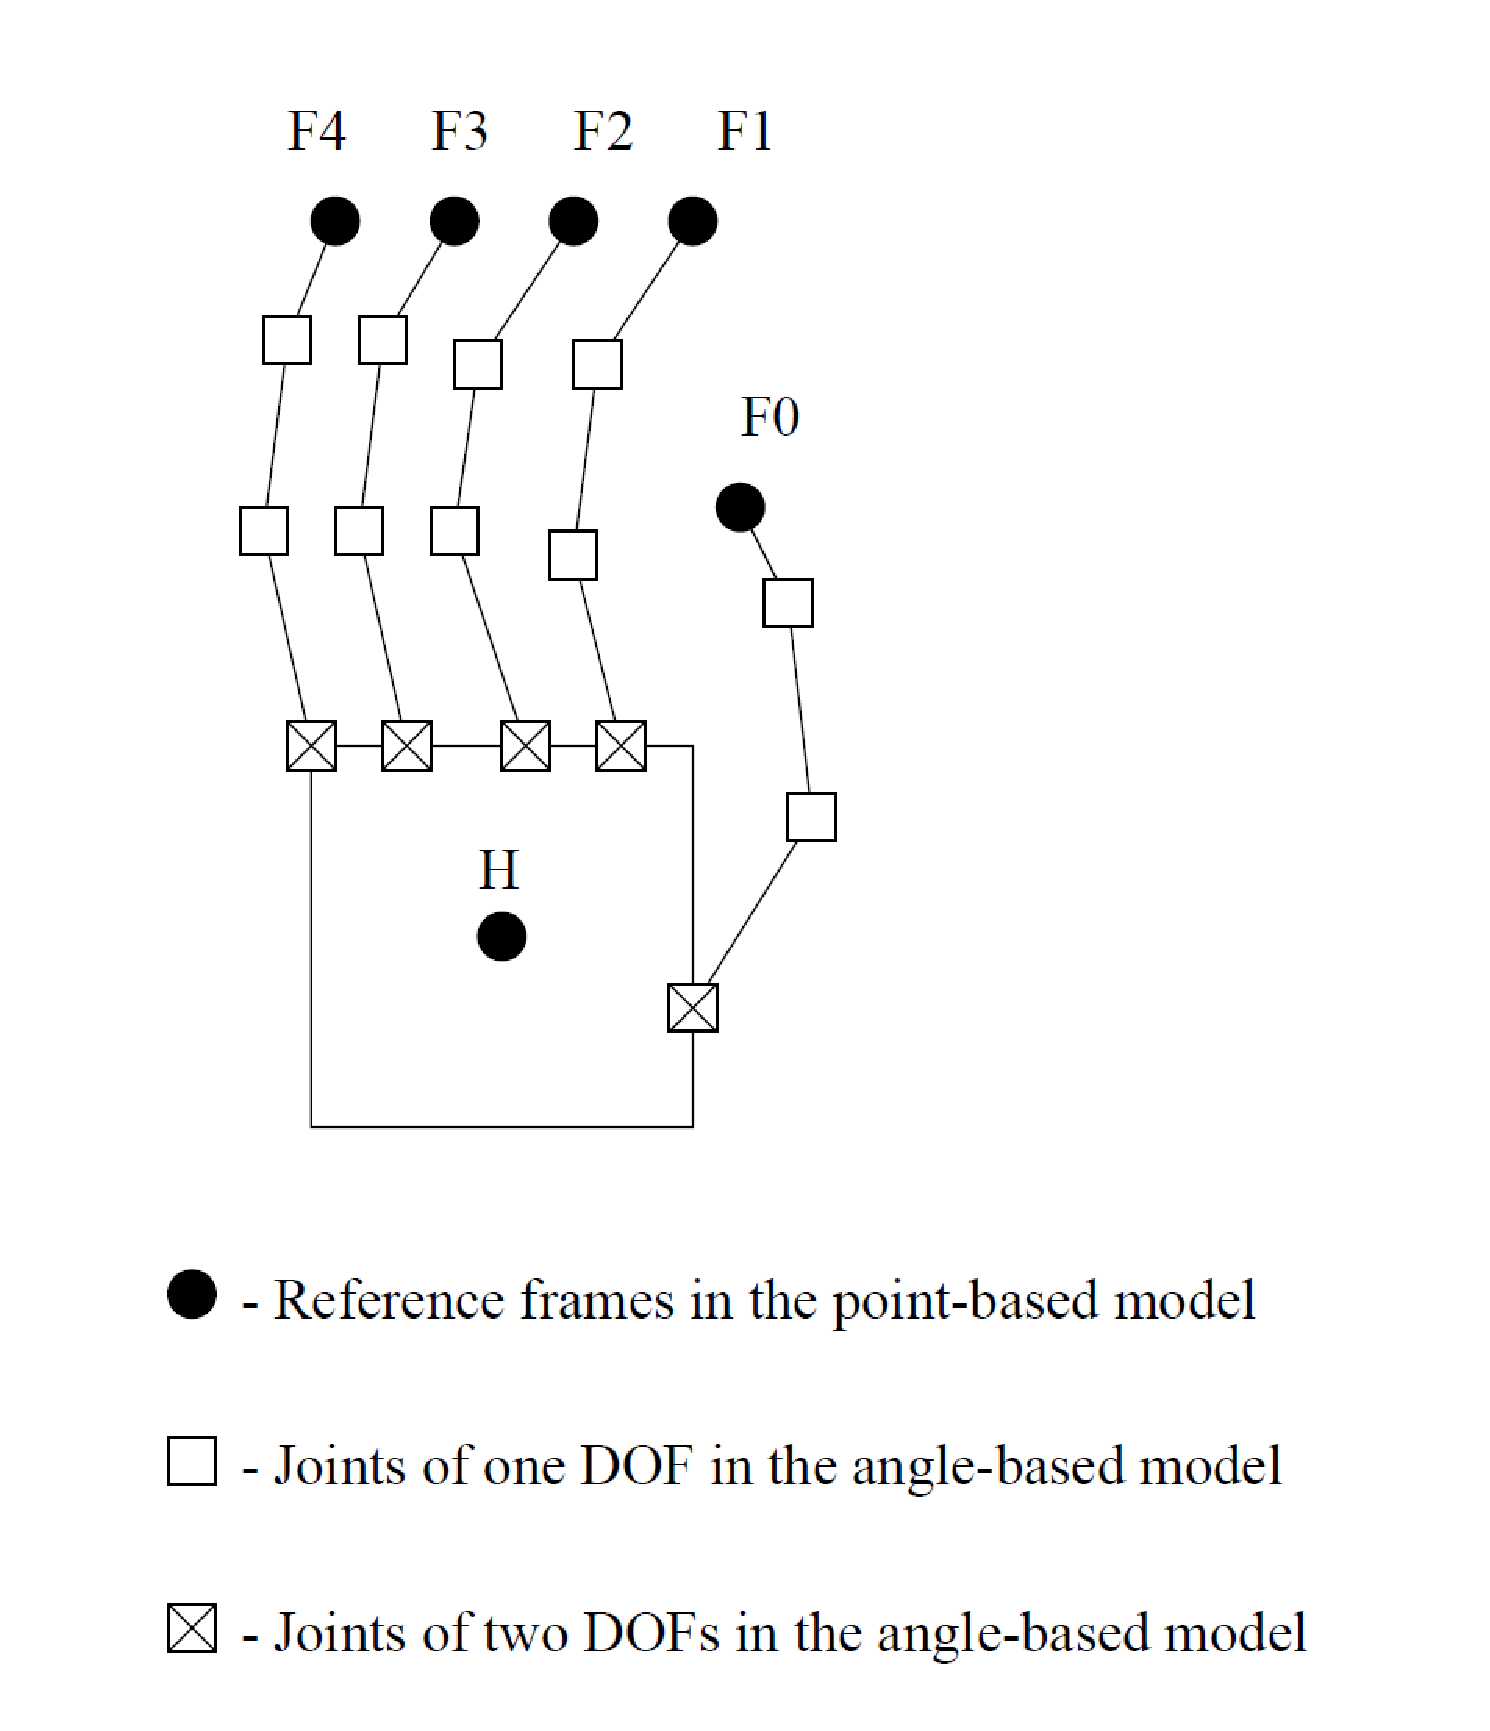
\includegraphics[width=\textwidth]{anglepoint}
\caption{Point-based and Angle-based Hand Models (from \cite{su1994logical}).}
\label{fig:anglepoint}
\end{figure}

The point-based hand model describes a hand posture as a set of 6 6DOF (position and orientation) points. 5 of these represent the finger tips, one represents the palm. In the angle-based hand model, a hand posture is described by the hand's joint angles. Depending on the literature, the joints in the hand have a total of 22 \cite{su1994logical} or 23 DOFs \cite{laviola1999survey}, differentiating in the DOFs of the \textit{trapeziometacarpal} joint (TMC, Figure \ref{fig:handAnatomyTotal}).
Even though the two models are almost interchangeable, the angle-based model was chosen, as it makes most computations of metric components trivial. A common simplification for angle-based hand models is to neglect the 2 DOFs, given by the \textit{metacarpocarpal} (MCC, Figure \ref{fig:handAnatomyTotal}) of the forth and fifth digit. This is done for example by the Leap, because the MCCs hardly move and are therefore are not noticeable for most applications. 
In conclusion, the implementation was based on a 21DOF angle based hand model, as it can be seen in Figure \ref{fig:anglehand}.

\begin{figure}[h]
\centering
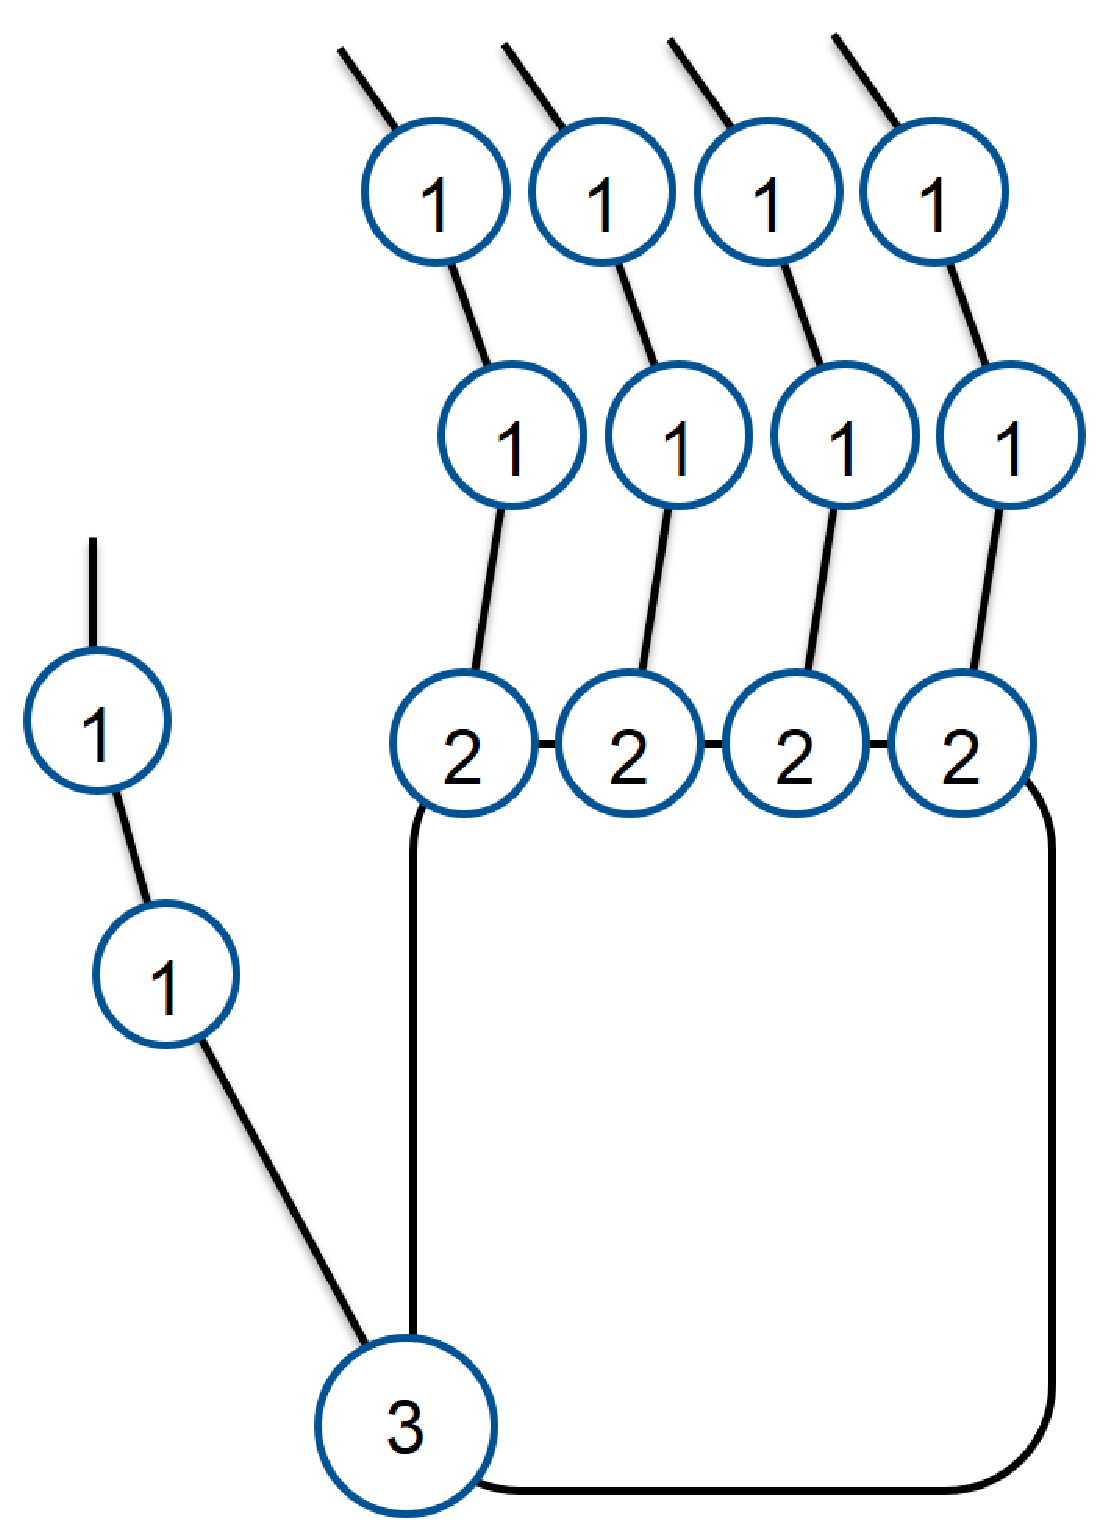
\includegraphics[width=0.40\textwidth]{anglehand}
\caption{Used Hand Model showing Joints with DOFs}
\label{fig:anglehand}
\end{figure}

The goal for the Unity implementation was to create a universally usable and flexible class structure for hand postures, thus the \texttt{AngleBasedHandModel} class was created. The class has a reference to a thumb object of class \texttt{AngleBasedThumbModel} and four enumerated fingers of class \texttt{AngleBasedFingerModel}. In addition the hands position and rotation are stored for debugging. The class also provides a function to calculate the mathematical Euclidean distance to another hand posture, a function to interpolate between two hand postures, a \texttt{toString} function and multiple functions for loading and storing hand postures as .CSV file. 

The \texttt{AngleBasedFingerModel} (and \texttt{AngleBasedThumbModel}) stores their 4 (and 5) DOFs as float angles. To ease computation the rotation of the MCP (and TMC) is redundantly stored as quaternion. Both classes also implement the same functions as \texttt{AngleBasedHandModel}. \texttt{AngleBasedFingerModel} additionally provides a function for computing the total flexion of a finger (Figure \ref{fig:hyperabduction}). The three classes are fully serializable to facilitate simple saving and loading of hand postures.
%TODO: add figure?
In order to obtain the hand posture data from the the Leap in realtime, a \texttt{HandObserver} script was attached to each Leap hand objects. The \texttt{HandObserver} extracted the hand posture data from the Leap and updated an \texttt{AngleBasedHandModel} object while taking the handedness into account.

\section{Hand Posture Classification}

In order to make sure, that the participant would hold the hand posture during the user study, some kind of hand posture classification system had to be implemented. While there are multiple different methods, that can be used for hand posture classification, the k-nearest neighbors (k-NN) algorithm has proven to be both suitable for hand posture classification and comparatively easy to implement \cite{gardner20143d}. 

The k-NN algorithm is a simple machine learning algorithm that can be applied to a multitude of problems with an n-dimensional feature vector. The basic idea is to test the membership of an object using training data. The membership of the vector is determined by the majority of it's k nearest neighbors. 

In the case of hand posture classification, we have a 21-dimensional feature vector according to our hand model. The implementation here was based on Nikolas Schneider's implementation, but was refactored to be more versatile in use. Basically the k-NN implementation has two main objectives:

\begin{enumerate}
	\item Data Collection
	\item Actual Posture Classification
\end{enumerate}

For \textbf{data collection} a set of training data, consisting of feature vectors with their classification has to be obtained. This was implemented by the \texttt{PostureDataHandler} class. The \texttt{PostureDataHandler} takes care of the training data, implemented as a list of \texttt{TrainingUnit} objects and provides functions to add and delete \texttt{TrainingUnit}s. A \texttt{TrainingUnit} consists of a \texttt{AngleBasedHandModel} object that is classified with a \texttt{Posture} enumerator. To achieve data persistence, the \texttt{PostureDataHandler} saves the data to the hard drive after every modification and automatically loads it when instantiated.

A \texttt{TrainingManager} scene (Figure \ref{fig:training}) was created that allows the user to manipulate the training data using a GUI. The user can inspect \texttt{TrainingUnit}s, that are visualized with a \texttt{OutputHand} built from Unity primitives. The \texttt{TrainingUnit}s are grouped by \texttt{Posture} and can be deleted individually or as group. In order to add \texttt{TrainingUnit}s the user has to choose the desired \texttt{Posture}, form the hand posture over the Leap and press a button. 

\begin{figure}[h]
\centering
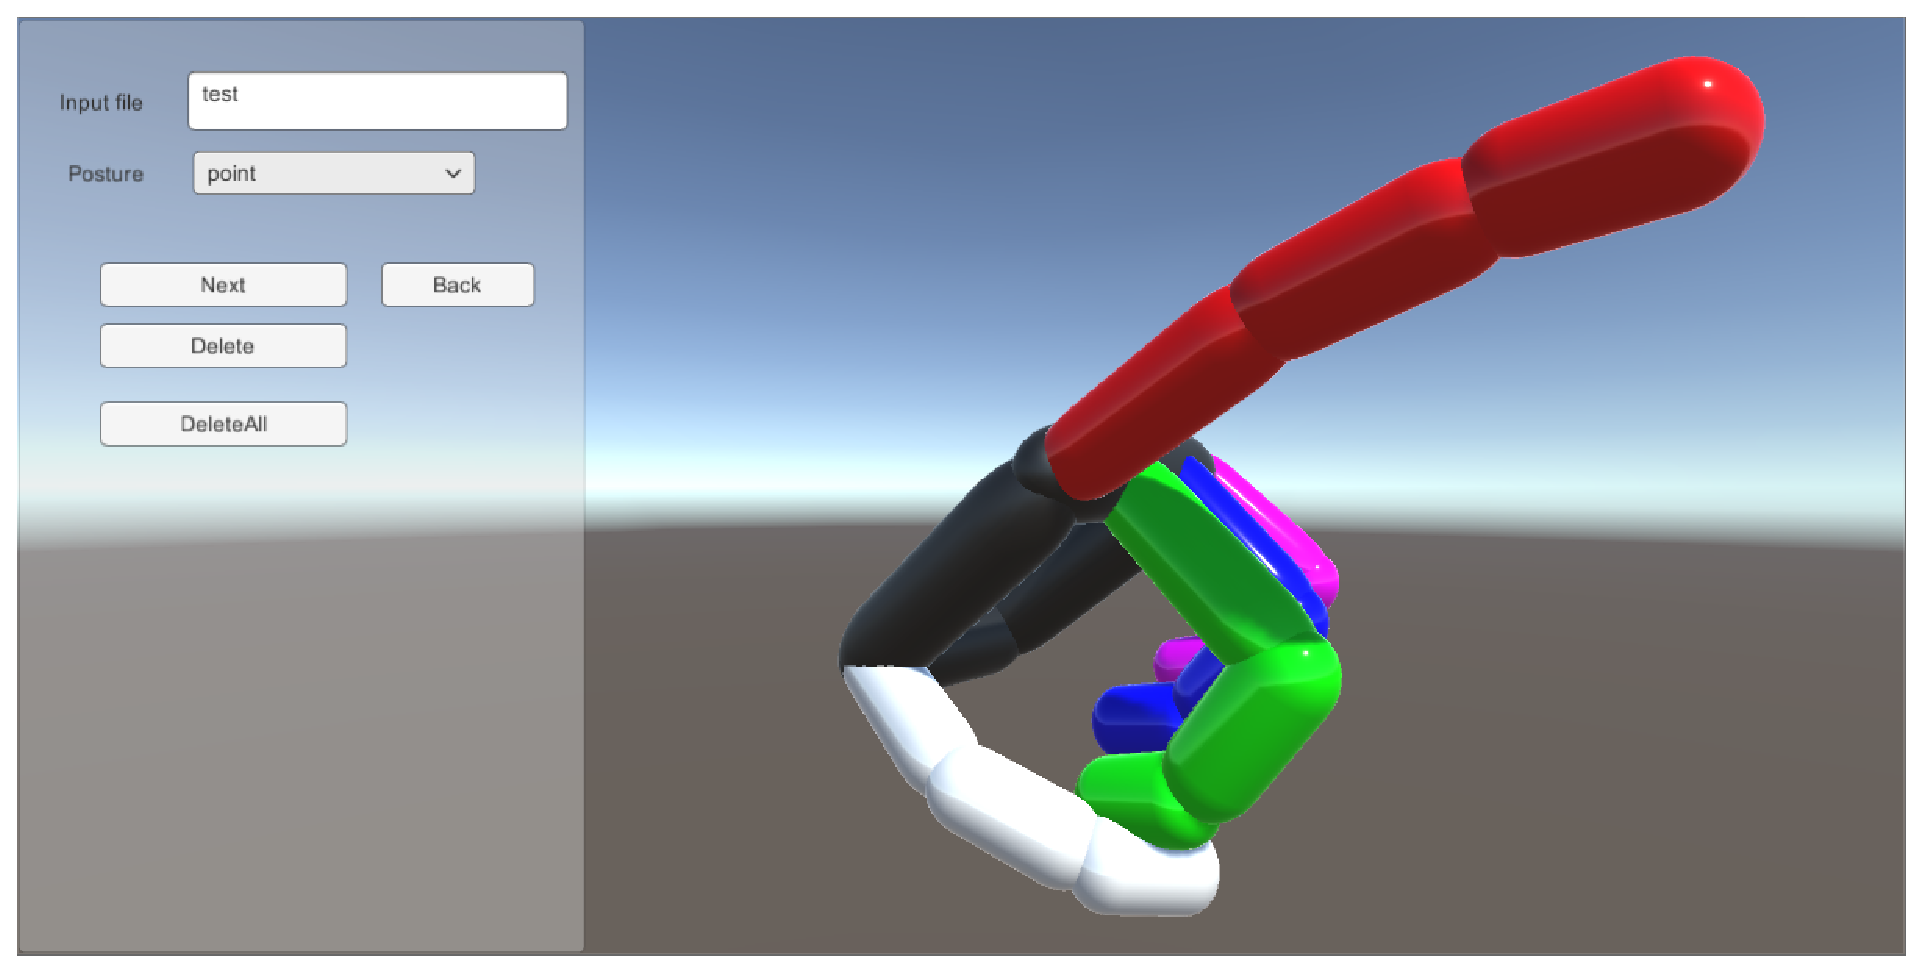
\includegraphics[width=\textwidth]{trianing}
\caption{Inspecting a pointing \texttt{TrainingUnit} in the \texttt{TrainingManager}.}
\label{fig:training}
\end{figure}

The \textbf{actual posture classification} classifies a hand posture based on the k nearest neighbors. For that, the distances of the hand posture to all training units has to be computed and the k closest have to be selected. In this case, k is set as the square root of the total training data size.

In the implementation this is handled by the \texttt{ThreadedKNN} class. As the name suggest, the classification is done in parallel to the main program using threads. Each frame the \texttt{ThreadedKNN} starts a new thread which receives the \texttt{AngleBasedHandModel} that needs to be classified. The thread receives a list of \texttt{PoseCompareObject}s from the \texttt{PostureDataHandler} containing the Euclidian distance of every \texttt{TrainingUnit} to the \texttt{AngleBasedHandModel} and its classifying \texttt{Posture}. The thread then sorts the list by distance and counts the occurrences of the different \texttt{Posture}s among the k nearest \texttt{PoseCompareObject}s. The \texttt{AngleBasedHandModel} is then classified as the most frequent \texttt{Posture} and the result is written back to the \texttt{ThreadedKNN} object.

In the context it was used, the k-NN implementation could differentiate between 10 postures with 50 recorded training samples each. The hand posture classification was performed on two hand robustly in real time without noticeable performance impact or lag. 


\section{Hand Posture Metrics}\label{chapter:handosturemetric}

Now that we have a representation for hand postures, the metric can be implemented. For that a \texttt{Comfort} and a \texttt{Discomfort} class were created. Both contain functions for computing the total metric value, the metric components for the whole hand and for the single fingers as well as functions for outputting the finger values to a .CSV file. 

\subsection{Comfort}

The only component, that is computed in \texttt{Comfort} is the distance to the RRP. Theoretically every DOF in the hand has an own RRP, that can be determined through experiments as done by Apostolico et al. \cite{apostolico2014postural}. However this turns out to be a costly and lengthy process, that had exceeded the focus of this thesis. Therefore some simplifications had to be made:

\begin{enumerate}
	\item The RRP will not be determined for every RRP separately but the whole hand simultaneously.
	\item The RRP will not be defined as a continuous range but as a discrete set of samples.
\end{enumerate}

In conclusion of this, the RRP would be defined as a set of relaxed hand postures (Figure \ref{fig:relaxed}). To implement this, the 50 samples of the "idle" \texttt{Posture} stored in the \texttt{PostureDataHandler} are used to define the hand's RRP. A correct implementation of the distance to the RRP would have been to compute the 21-dimensional bounding volume of the RRP, test a hand posture for collision with the volume and calculate the minimum distance to the volume. Again as a simplification, only the minimum Euclidean distance to any sample of the RRP set are computed. Strictly seen, a hand posture within the RRP could have a RRP value \begin{math}\not= 0\end{math}, 
but early tests showed the error to be negligibly small.
The result were two functions, one that calculated the minimum distance to the RRP for the whole hand, one that calculated it for every single finger individually.

\subsection{Discomfort}

In \texttt{Discomfort} the three discomfort components were computed: inter finger angles, hyperextension and abduction.

For the whole-hand computation of inter finger angles, initially only the absolute flexing differences between the fingers were added up. However, it showed early that the anatomical differences between the individual fingers influence the inter finger angle discomfort so severely, that they already have to be compensated in the naive metric. Most of all, the ring finger showed to be incapable of having large flexion differences to its adjacent neighbors. However this only stands out when the ring finger has to stick out between its neighbors, not when it is between them. Therefore a ring finger bonus was added, that was computed as follows: 
\vspace{5pt}
\begin{center}
\texttt{Mathf.Abs((fingers[middle].getTotalFlexion() - fingers[ring].getTotalFlexion() ) - \\
(fingers[ring].getTotalFlexion() - fingers[pinky].getTotalFlexion()));}
\end{center}
\vspace{5pt}
This way, the ring bonus only occurs, when the ring finger sticks out between it's neighbors. The ring bonus is multiplied with a weighting coefficient, which was estimated to be 1.3.

For computing the single-finger values, index and pinky receive the angle differences to their only neighbors while the middle and ring finger values are computed similarly to the ring bonus. 

The computation of the hyperextension is more straight forward. Hyper-extended fingers due to the nature of our hand model have negative extension angles in the MCP. Consequently the single finger hyper extension values are the absolute extension angle of the MCP if the finger is hyper-extended otherwise 0. 

Due to the angle-based hand model, computing the single finger abduction component, comes down calculating the absolute of the fingers MCP abduction angle.

For both hyperextension and finger abduction the whole hand metric value is simply the sum of the single finger values. 

To get the total naive discomfort value, the 3 whole hand values are weighted with their importance coefficients and afterwards added up.

\section{Random Hand Generator}

One potential weak spot, when comparing and examining hand postures is the process of choosing the hand postures to compare. In the context of this thesis, as many diverse hand postures as possible had to be compared in order to get universally valid picture. To solve this, one possible approach is to randomly generate hand postures. 
For this, a \texttt{RandomHandGenerator} was created. The class provides a function that returns a random \texttt{AngleBasedHandModel}. Internally the function again chooses from 4 different random hand generators randomly. The different functions are: \texttt{createRandomRandom(), createRandomFromSaved(), createRandomFromSavedMorph(), createRandomProcedural()}. 

The \texttt{createRandomRandom()} function was the first method to be created. It uses maximum and minimum joint angle values, defining the Range of Motion (ROM) \cite{apostolico2014postural}. For each individual finger an individual flexion and abduction within the predefined ROM is computed.

In the \texttt{createRandomFromSaved()} a hand posture is composed by randomly picking finger postures from the training data. For every finger a random \texttt{TrainingUnit} is picked from the \texttt{PostureDataHandler} and that specific finger is taken over by the new random hand. This way, many interesting hand posture combinations can be created of the 10 different training data postures.

\texttt{createRandomFromSavedMorph()} also works using the training data. For the creation of a random hand, two random \texttt{TrainingUnits} are again picked. The resulting hand is created, by interpolating the two hand postures, with the weight varying between the fingers. 

Finally the \texttt{createRandomProcedural()} contains a set of predefined finger states, similar as described in the paper of Su et al. \cite{su1994logical}. For the thumb the states \texttt{Under, Downward, Aligned} and \texttt{Sideways} are defined, the remaining fingers have the possible states \texttt{HyperExtended, Flat, Fist} and \texttt{ForwardFist}. Each of the hand's fingers is assigned one state randomly and a random global abduction value is generated, defining the total fanning of the fingers, before assembling the actual hand posture from predefined finger configurations corresponding to the finger states.

To guarantee a homogenous distribution of comfort and discomfort among the randomly generated hand postures, a random range of possible naive comfort/discomfort metric values for the hand posture is defined beforehand. The random hand generation process is repeated until the calculated naive metric value of the hand posture lies within the specified range.

\section{User Study Tests}

For investigating the main questions of the thesis, a test environment had to be created. In order to verify and to improve the metric, the idea was to let participants rate different hand postures and compare the ratings with the computed metric values. Additionally, the objective was to show the impact of comfort and discomfort on precision and performance in different tasks, for that a target shooting test and a line tracing test were implemented.
The user study was designed for a seated participant in front of a desk, with the elbow of the dominant hand resting on the edge. For interaction a controller and a monitor were placed on the desk. Additionally a Leap Motion controller was attached to the desk.  

\subsection{Hand Posture Evaluation}


\begin{figure}
\centering
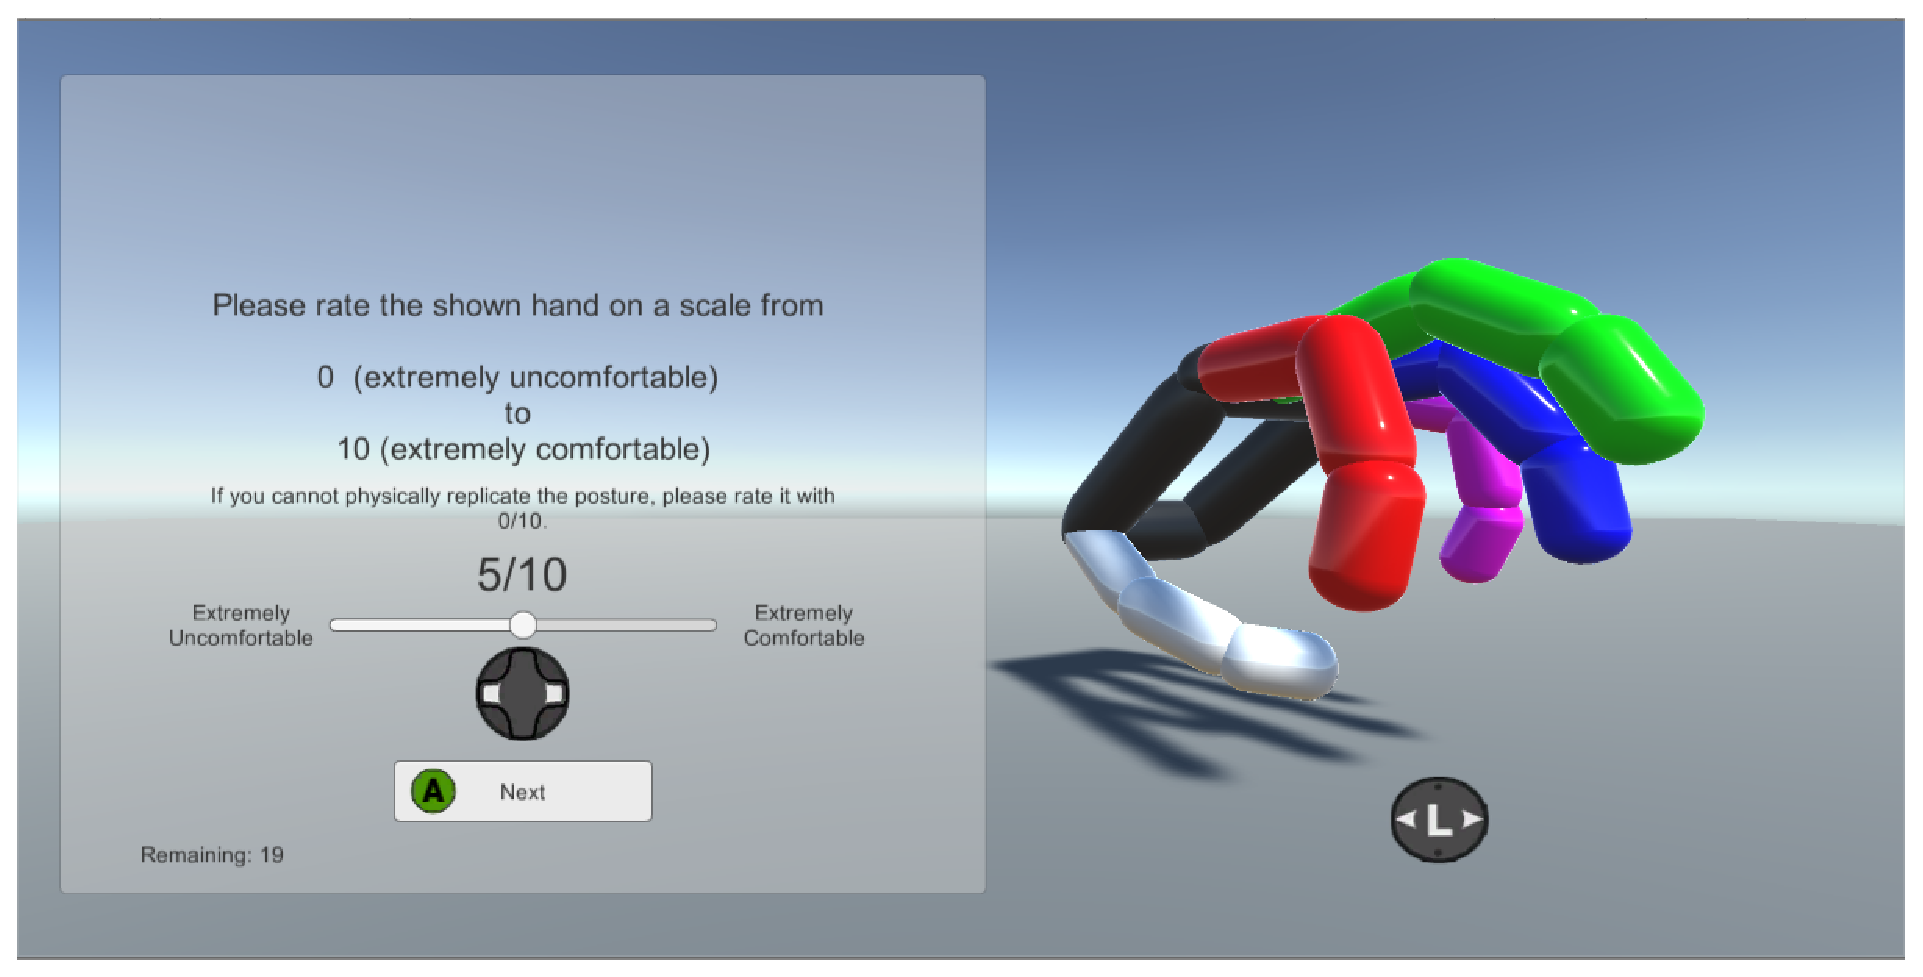
\includegraphics[width=\textwidth]{evaluation}
\caption{The Hand Posture Comfort Evaluation Scene.}
\label{fig:evaluation}
\end{figure}

For the hand posture evaluation, a \texttt{UserStudyComfortEvaluation} scene was created (Figure \ref{fig:evaluation}). To begin the test, a random hand posture is generated and visualized using the \texttt{OutputHand} known from the \texttt{TrainingManager} scene. Afterwards the participant has to imitate the hand posture and rate the hand posture on an intuitive comfort/discomfort scale ranging from 0 (extremely uncomfortable) to 10 (extremely comfortable). If the participant is unable to mimic the hand posture due to its complexity, the posture was supposed to be rated with a 0. After confirming his or her choice, the results are logged to a .CSV file. For that, the naive and improved metric components are computed and logged together with the participants rating and name. In addition the whole randomly generated hand is logged, in order to be able to do further calculations later on if necessary.

Before the first hand posture evaluation the participant is shown two different randomly generated hand postures, to get a reference on what to expect in terms of comfort and discomfort. The first hand posture is supposed to be a relaxed one that could be rated with a 10, therefore with a metric value close to 0. The second hand posture should represent an extremely uncomfortable hand posture resulting in a 0 rating, therefore the metric value should be as high as possible.

\subsection{Precision and Performance Tests}

Before the target shooting and the line tracing test, the participant is again shown a randomly generated hand posture, that is meant to be tested. Again the user has to mimic the hand posture with the dominant hand and again the user has to rate the hand. After rating, the subject has to hold his hand over the Leap while holding the posture. In order to track the hand posture during the tests, the hand posture has to be learned by the k-NN. For that the Leap records 50 samples of the hand and the hand posture data is saved as \texttt{TrainingUnit}s by the \texttt{PostureDataHandler}. 

After that the actual tests starts. If the participants brake the hand posture they are kindly asked to correct it. During both tests the participants are shown a visualization of the given hand posture in the bottom right corner as a reminder. They have to perform different tasks using their dominant hand while maintaining the hand posture. 
For that, the subjects are shown a minimalistic representation of their hand position that was recorded with the Leap. In favor of comparability, the pointing direction is universally set independent of the hand posture as the forward direction of the hand base, and is visualized with a laser beam (Figure \ref{fig:target} and \ref{fig:line}). 

\subsection{Target Shooting Test}

The target shooting test was chosen to test the performance impact in context of quick punctual pointing. This specific test was chosen due to its similarity to real world tasks, such as giving a robot quick spatial commands or commanding units to perform some action somewhere in space in a RTS game. To implement this, the \texttt{UserStudyTargetShooting} scene was created (Figure \ref{fig:target}).

\begin{figure}
\centering
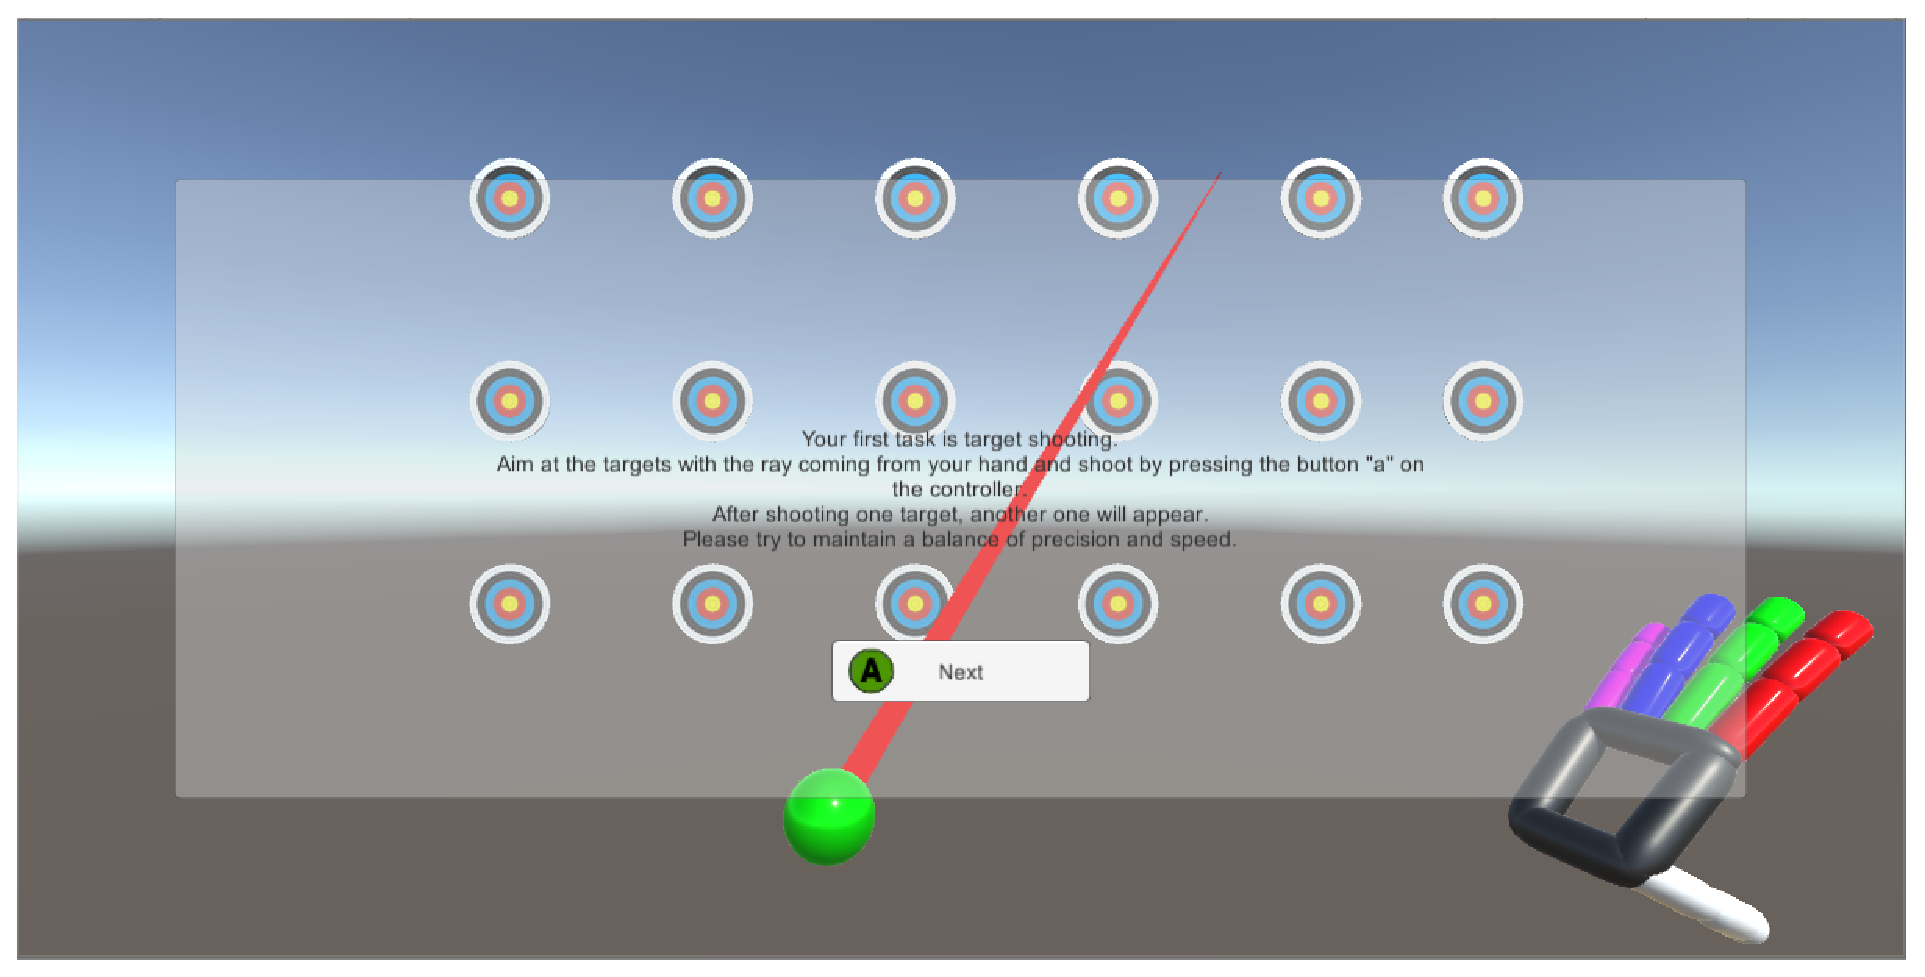
\includegraphics[width=\textwidth]{targetshootingt}
\caption{The Target Shooting Test.}
\label{fig:target}
\end{figure}

The scene features a total of 18 targets which appear individually in a random order. The participant then has to aim down the individual targets with their hand and shoot them with the press of a button.
Once a target is hit, the distance of the hit to the target's center is computed as a metric for accuracy. The accuracy value, the time to hit as well as the different metric components and the whole hand are then logged in a .CSV file.  

When the participants brake the hand posture, shooting is locked, until the hand posture is corrected. 

\subsection{Line Tracing Test}

The line tracing test was chosen due to its similarity to real world tasks such as drawing a route to be traversed by a robot or patrolled by units in a RTS.
For this, the \texttt{UserStudyLineTracing} scene was created (Figure \ref{fig:line}).

\begin{figure}
\centering
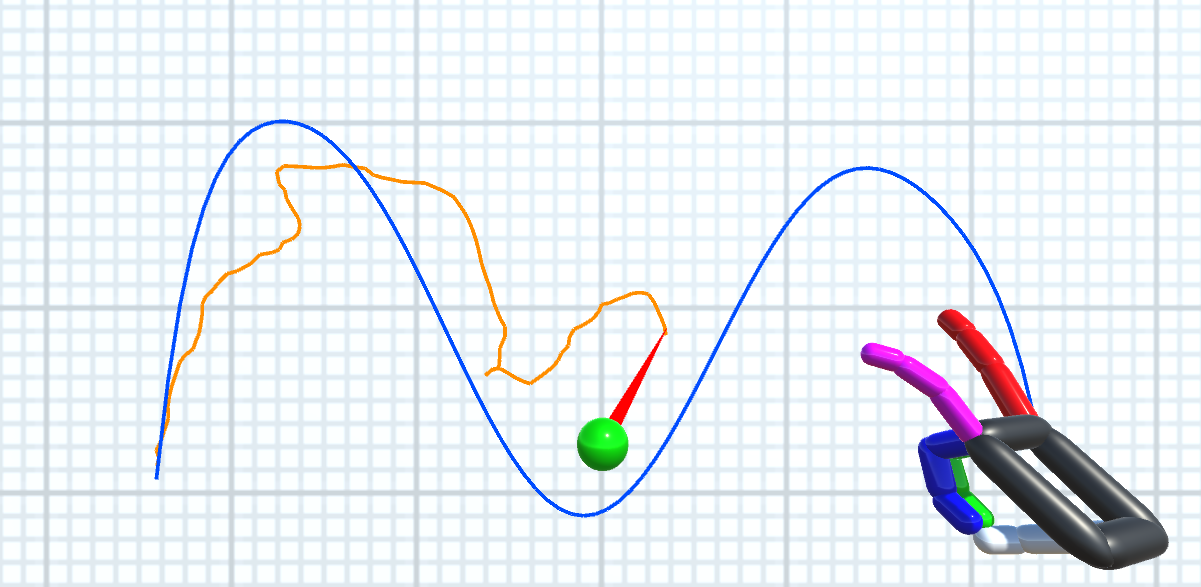
\includegraphics[width=\textwidth]{linetracing}
\caption{The Line Tracing Test.}
\label{fig:line}
\end{figure}

In the test, the participant is shown a blue curve on a drawing plane, that has to be traced. For that the user has to use the ray to draw his own line on the drawing plane as close to the given curve as possible by holding a controller button. If the participant brakes the hand posture, drawing is interrupted, if the user releases the drawing button, the test is ended after a certain timeout.
After the test is ended, the total accuracy is calculated and is logged together with the total task completion time, hand posture metric values and the whole hand in a .CSV file.

The curves were implemented as discrete sets of \texttt{LinePoint}s that are connected to their neighbors with line segments. In order to get a smooth curve 12 random points are generated on the drawing plane and a bezier curve is fitted through them. The bezier curve is then discretized in 75 \texttt{LinePoint}s. For drawing the line, a \texttt{LinePoint} is set at the starting point and a second is moved with the ray on the drawing plane. As soon as the second \texttt{LinePoint} moves too far away from the previous \texttt{LinePoint}, it is fixed to its position and a new \texttt{LinePoint} is added in and moved further instead.

The accuracy can be determined by calculating the average minimum distance of every drawn \texttt{LinePoint} to the given curve defined by its \texttt{LinePoint}s. The same is done the other way around and added up to the total line accuracy value. 

\subsection{The User Study Management}

In order to automate the user study process, a \texttt{UserStudyDevScreen} scene was added in (Figure \ref{fig:devscreen}). The scene shows a GUI, that can be used to configure a whole user study for one participant. The experimenter can set the name of the participant, his handedness and choose a \texttt{Pose} to be overwritten by the users hand recordings. Further it can be selected which of the three user study test have to be performed and how often these will be repeated for different hand postures. 

\begin{figure}
\centering
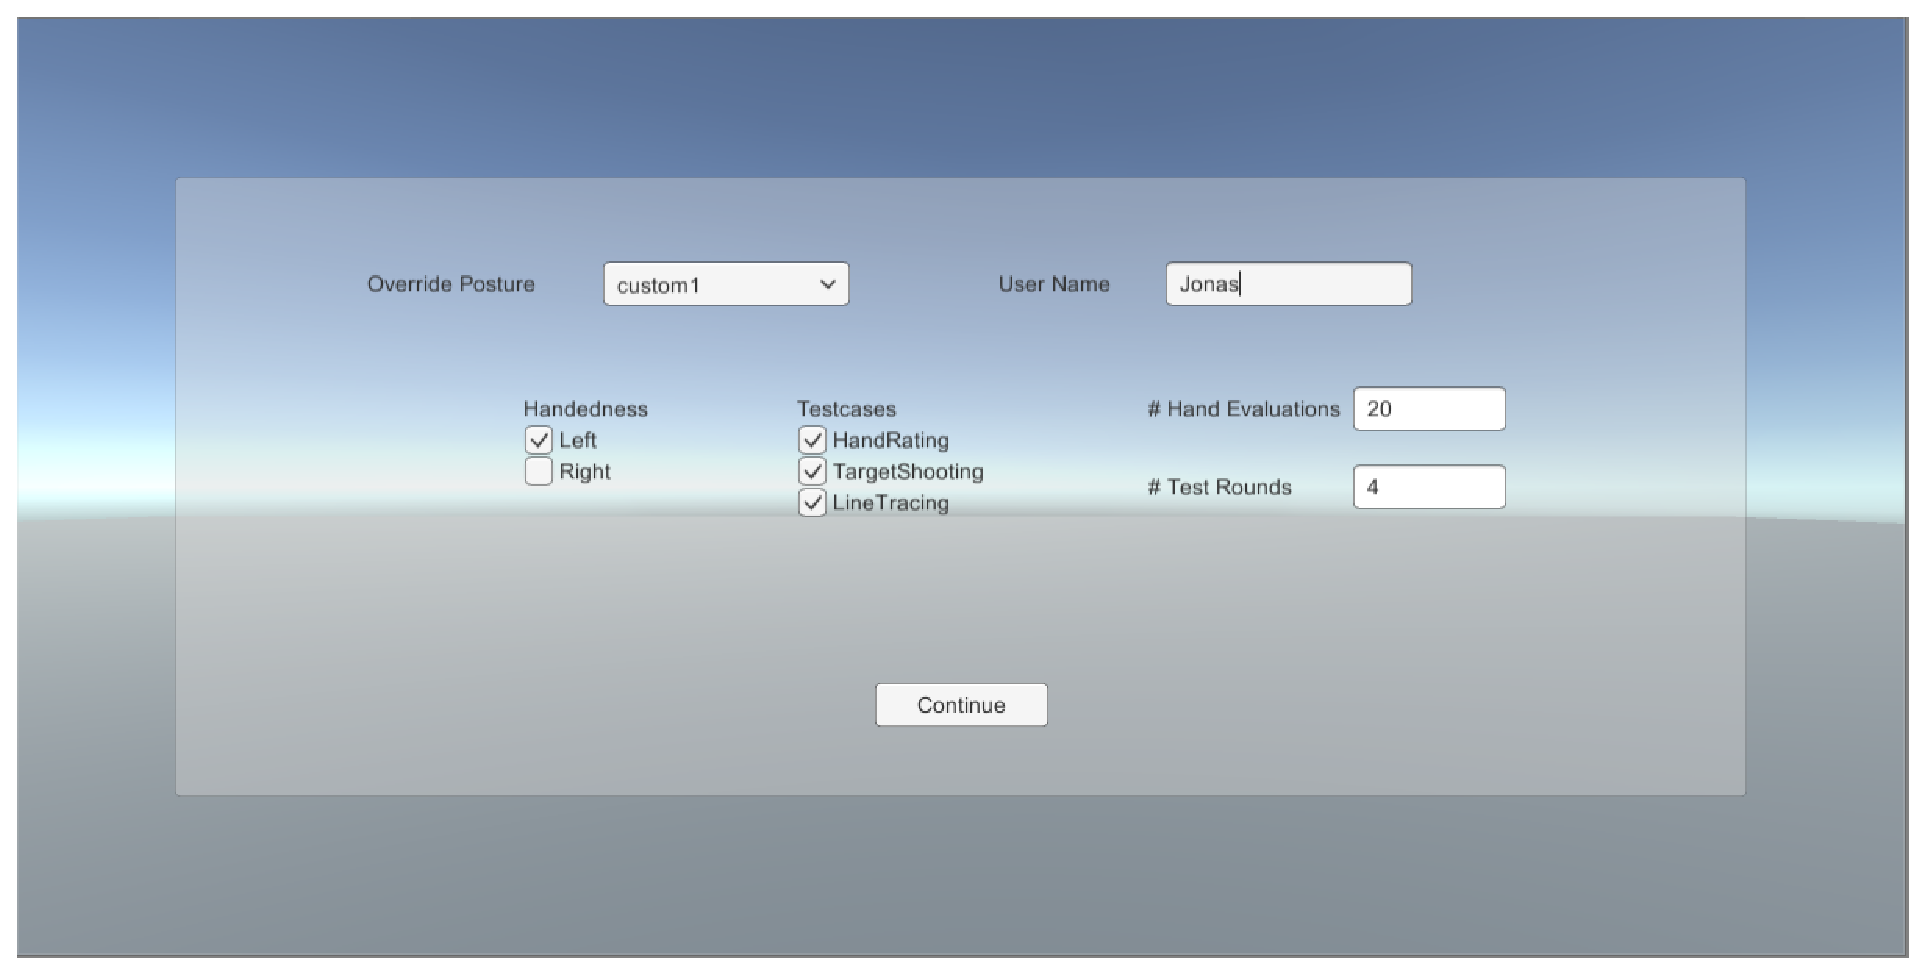
\includegraphics[width=\textwidth]{devscreen}
\caption{The User Study DevScreen.}
\label{fig:devscreen}
\end{figure}

After confirming the setting, the user study will start with the desired number of hand posture evaluations and automatically switch to the precision and performance tests. After finishing the complete user study, the participant is shown an ending screen, thanking him for participating in the study and giving him the opportunity to play around with the standard Leap hand visualization. 

\section{Stumbling Blocks}

During implementation, a variety of unexpected problems occurred and different concepts turned out to not work in this context as expected. The following section describes different stumbling blocks that can commonly be found in similar contexts or were severe threats to the project. 

\subsection{Serialization and Normalization of Vector3 and Quaternions}

Since a \texttt{BinaryFormatter} is used for saving and loading the training data in the \texttt{PostureDataHandler}, all saved objects have to be serializable. For this \texttt{TrainingUnit} has to be serializale, consequently a \texttt{AngleBasedHandModel} and a \texttt{AngleBasedFinger}- and -\texttt{ThumbModel} have to be serializable. As \texttt{float}s and \texttt{Enum}s are both serializable, the only problems were \texttt{Vector3} and \texttt{Quaternion}, the standard Unity classes, that for some reason are not serializable. The only solution for this was to create a custom struct for vectors and quaternions. 

Thus, the \texttt{sVector3} and \texttt{sQuaternions} were created. Both \texttt{struct}s basically implement their unserializable counterparts, in both cases operators were defined to enable implicit typecasting to the unserializable form and back. For logging, both \texttt{struct}s also received additional functions for printing and parsing into .CSV files.

When extracting the MCP and TMC angles (Figure \ref{fig:handAnatomyTotal}) of the fingers, it is necessary to compute the relative rotations of the finger joints compared to their parents. The first idea, was to use the different functions of the Unity \texttt{Transform} class, but it turned out, that this class is unable to be instantiated without being a component of a game object. Therefore direct quaternion multiplication was used, as defined in the standard Unity class. After a while it became clear, that the standard quaternion multiplication would not automatically normalize the result, which caused several bugs when trying to do further computations with the \texttt{Quaternion}s. Obviously the standard unity functions do not check if a \texttt{Quaternion} is normalized before doing further computations. 

The bug was even harder to track, as it could not be visualized due to the \texttt{Transform} class automatically normalizing a \texttt{Quaternion} when applied to it as rotation.

As a consequence of this, the \texttt{sQuaternion} also received a function for normalization and length computation, as the standard \texttt{Quaternion} class implements neither.

Finally, creating a ambidextrous hand posture classification environment required to be able to transform a left handed hand posture to a right handed one and vice versa. Thus, functions for mirroring \texttt{sQuaternion}s around different axes had to be implemented as \texttt{Quaternion} did not provide any.

\subsection{Leap Tracking}

The Leap Motion Orion SDK was a big step forward for the tracking of the Leap. It enables tracking of awkward postures such as pinching, that were not possible to track before, it improves the finger pose estimation for occluded fingers and overall massively improves the range and robustness at different lighting conditions. However, due to its intended field of use, the Leap tracking is focused on quick and fluent hand and finger tracking, that provides the precision needed to create a reasonable visual parity. However, for contexts that require high precision, the Leap struggles to deliver usable data. 

While this characteristic of the Leap was no problem for the hand posture classification, it lead to unacceptable impact for pointing, especially for unconventional hand postures. Using the ray to aim down targets or to trace a line magnified the inaccuracies of the hand tracking, resulting in accuracy loss in the user studies. Because the tracking inaccuracies exceeded the expected accuracy loss by hand postures, an alternative hand tracking solution had to be found.

For precise hand tracking a optical outside-in solution was used, the ART system. Using four cameras the system can detect a marker attached to the back of the user's hand (as seen in Figure \ref{fig:baschde}). By attaching a marker to the user study desk, the ART hand position could be calibrated to the same coordinate system as used by the Leap. The tracking data of the ART was implemented to only be used for hand rotation and position in the target shooting and line tracing task. When ART tracking fails for some reason, the system automatically switches back to the legacy Leap hand tracking.  

The result was a much higher tracking precision that allows meaningful user accuracy observation.  

However the need for the user to wear a hand tracker yielded yet another problem. The tracker's black rubber strap, wrapped around the user's hand was visible for the Leap. In some cases this inferred with the hand detection, causing the Leap to detect a small closed fist in the lower half of the hand. However, this problem could be solved by occluding the strap with something with a similar IR signature as skin. For the user study this was realized by wrapping a paper towel around the strap. 

\subsection{Hand Posture Detection}

The hand posture detection as implemented by the k-NN algorithm was supposed to differentiate between a relatively small set of predefined hand postures. Through the addition of the random hand generator, samples of random hand postures were added with a "custom" \texttt{Posture} to the training data set. Problems occurred, when the randomly generated posture was similar or identical to a predefined hand posture by coincidence. This caused problems in the user studies, when the predefined posture was detected instead of the custom one and the user was notified to correct his hand posture even though he had the right hand posture. 

As a consequence the misuse of the k-NN was ended, instead only the minimum Euclidean distance to the "custom" \texttt{TrainingUnit}s is computed, similar as it is computed for the RRP component. If the minimum distance is smaller than a certain threshold, the hand is considered to hold the hand posture.